\section{Introduction}

Powered by large language models (LLMs; \citealt{openai2024gpt4o,team2023gemini,jiang2024mixtral,chang2024survey}), user-facing AI systems (such as ChatGPT) have become increasingly capable of performing complex tasks such as accurately responding to user queries, solving math problems, and generating code.
In particular, AI \emph{agents}, systems that can perceive and act upon the external environment, have recently received ever-increasing research focus.
They are moving towards performing complex tasks such as developing software \citep{jimenez2024swebench},
navigating real-world websites \citep{zhou2023webarena}, doing household chores \citep{ahn2022can}, or even performing scientific research \citep{boiko2023autonomous,tang2024prioritizing}. 

As AI agents become capable of tackling complex problems, their development and evaluation have also become challenging. 
There are numerous recent efforts in creating open-source frameworks that facilitate the development of agents \citep{hong2023metagpt,chen2024autoagents,wu2023autogen}.
These agent frameworks generally include: 1) \textbf{interfaces} through which agents interact with the world (such as JSON-based function calls or code execution), 2) \textbf{environments} in which agents operate, and 3) \textbf{interaction mechanisms} for human-agent or agent-agent communication.
These frameworks streamline and ease the development process in various ways (\tref{tab:comparison}, \sref{sec:related_work}).

When designing AI agents, we can also consider how \emph{human} interacts with the world.
The most powerful way in which humans currently interact with the world is through \emph{software} -- software powers every aspect of our life, supporting everything from the logistics for basic needs to the advancement of science, technology, and AI itself.
Given the power of software, as well as the existing tooling around its efficient development, use, and deployment, it provides the ideal interface for AI agents to interact with the world in complex ways.
However, building agents that can effectively develop software comes with its own unique challenges.
How can we enable agents to effectively \emph{create and modify code in complex software systems}?
How can we provide them with tools to \emph{gather information on-the-fly} to debug problems or gather task-requisite information?
How can we ensure that development is \emph{safe and avoids negative side effects} on the users' systems?

In this paper, we introduce \projname (\emph{f.k.a.} OpenDevin), a community-driven platform designed for the development of generalist and specialist AI agents that interact with the world through software.%
\footnote{While initially inspired by AI software engineer Devin \citep{cognition_devin}, \projname has quickly evolved to support much wider range of applications beyond software engineering through diverse community contributions.}
It features:
\begin{itemize}[noitemsep,topsep=0pt,parsep=2pt,partopsep=0pt,leftmargin=18pt]
\item[(1)] An \textbf{interaction mechanism} which allows user interfaces, agents, and environments to interact through an \emph{event stream} architecture that is powerful and flexible (\sref{sec:agent-abstraction}).
\item[(2)] A \textbf{runtime environment} that consists of a docker-sandboxed operating system with a bash shell, a web browser, and IPython server that the agents can interact with (\sref{sec:agent-runtime}).
\item[(3)] An \textbf{interface} allowing the agent to interact with the environment in a manner similar to actual software engineers (\sref{sec:agent-skills}). We provide the capability for agents to a) create and edit complex software, b) execute arbitrary code in the sandbox, and c) browse websites to collect information.
\item[(4)] \textbf{Multi-agent delegation}, allowing multiple specialized agents to work together (\sref{sec:agent-delegation}).
\item[(5)] \textbf{Evaluation framework}, facilitating the evaluation of agents across a wide range of tasks (\sref{sec:evaluation}).

\end{itemize}


\begin{figure}
\centering
\vspace{-0.2cm}
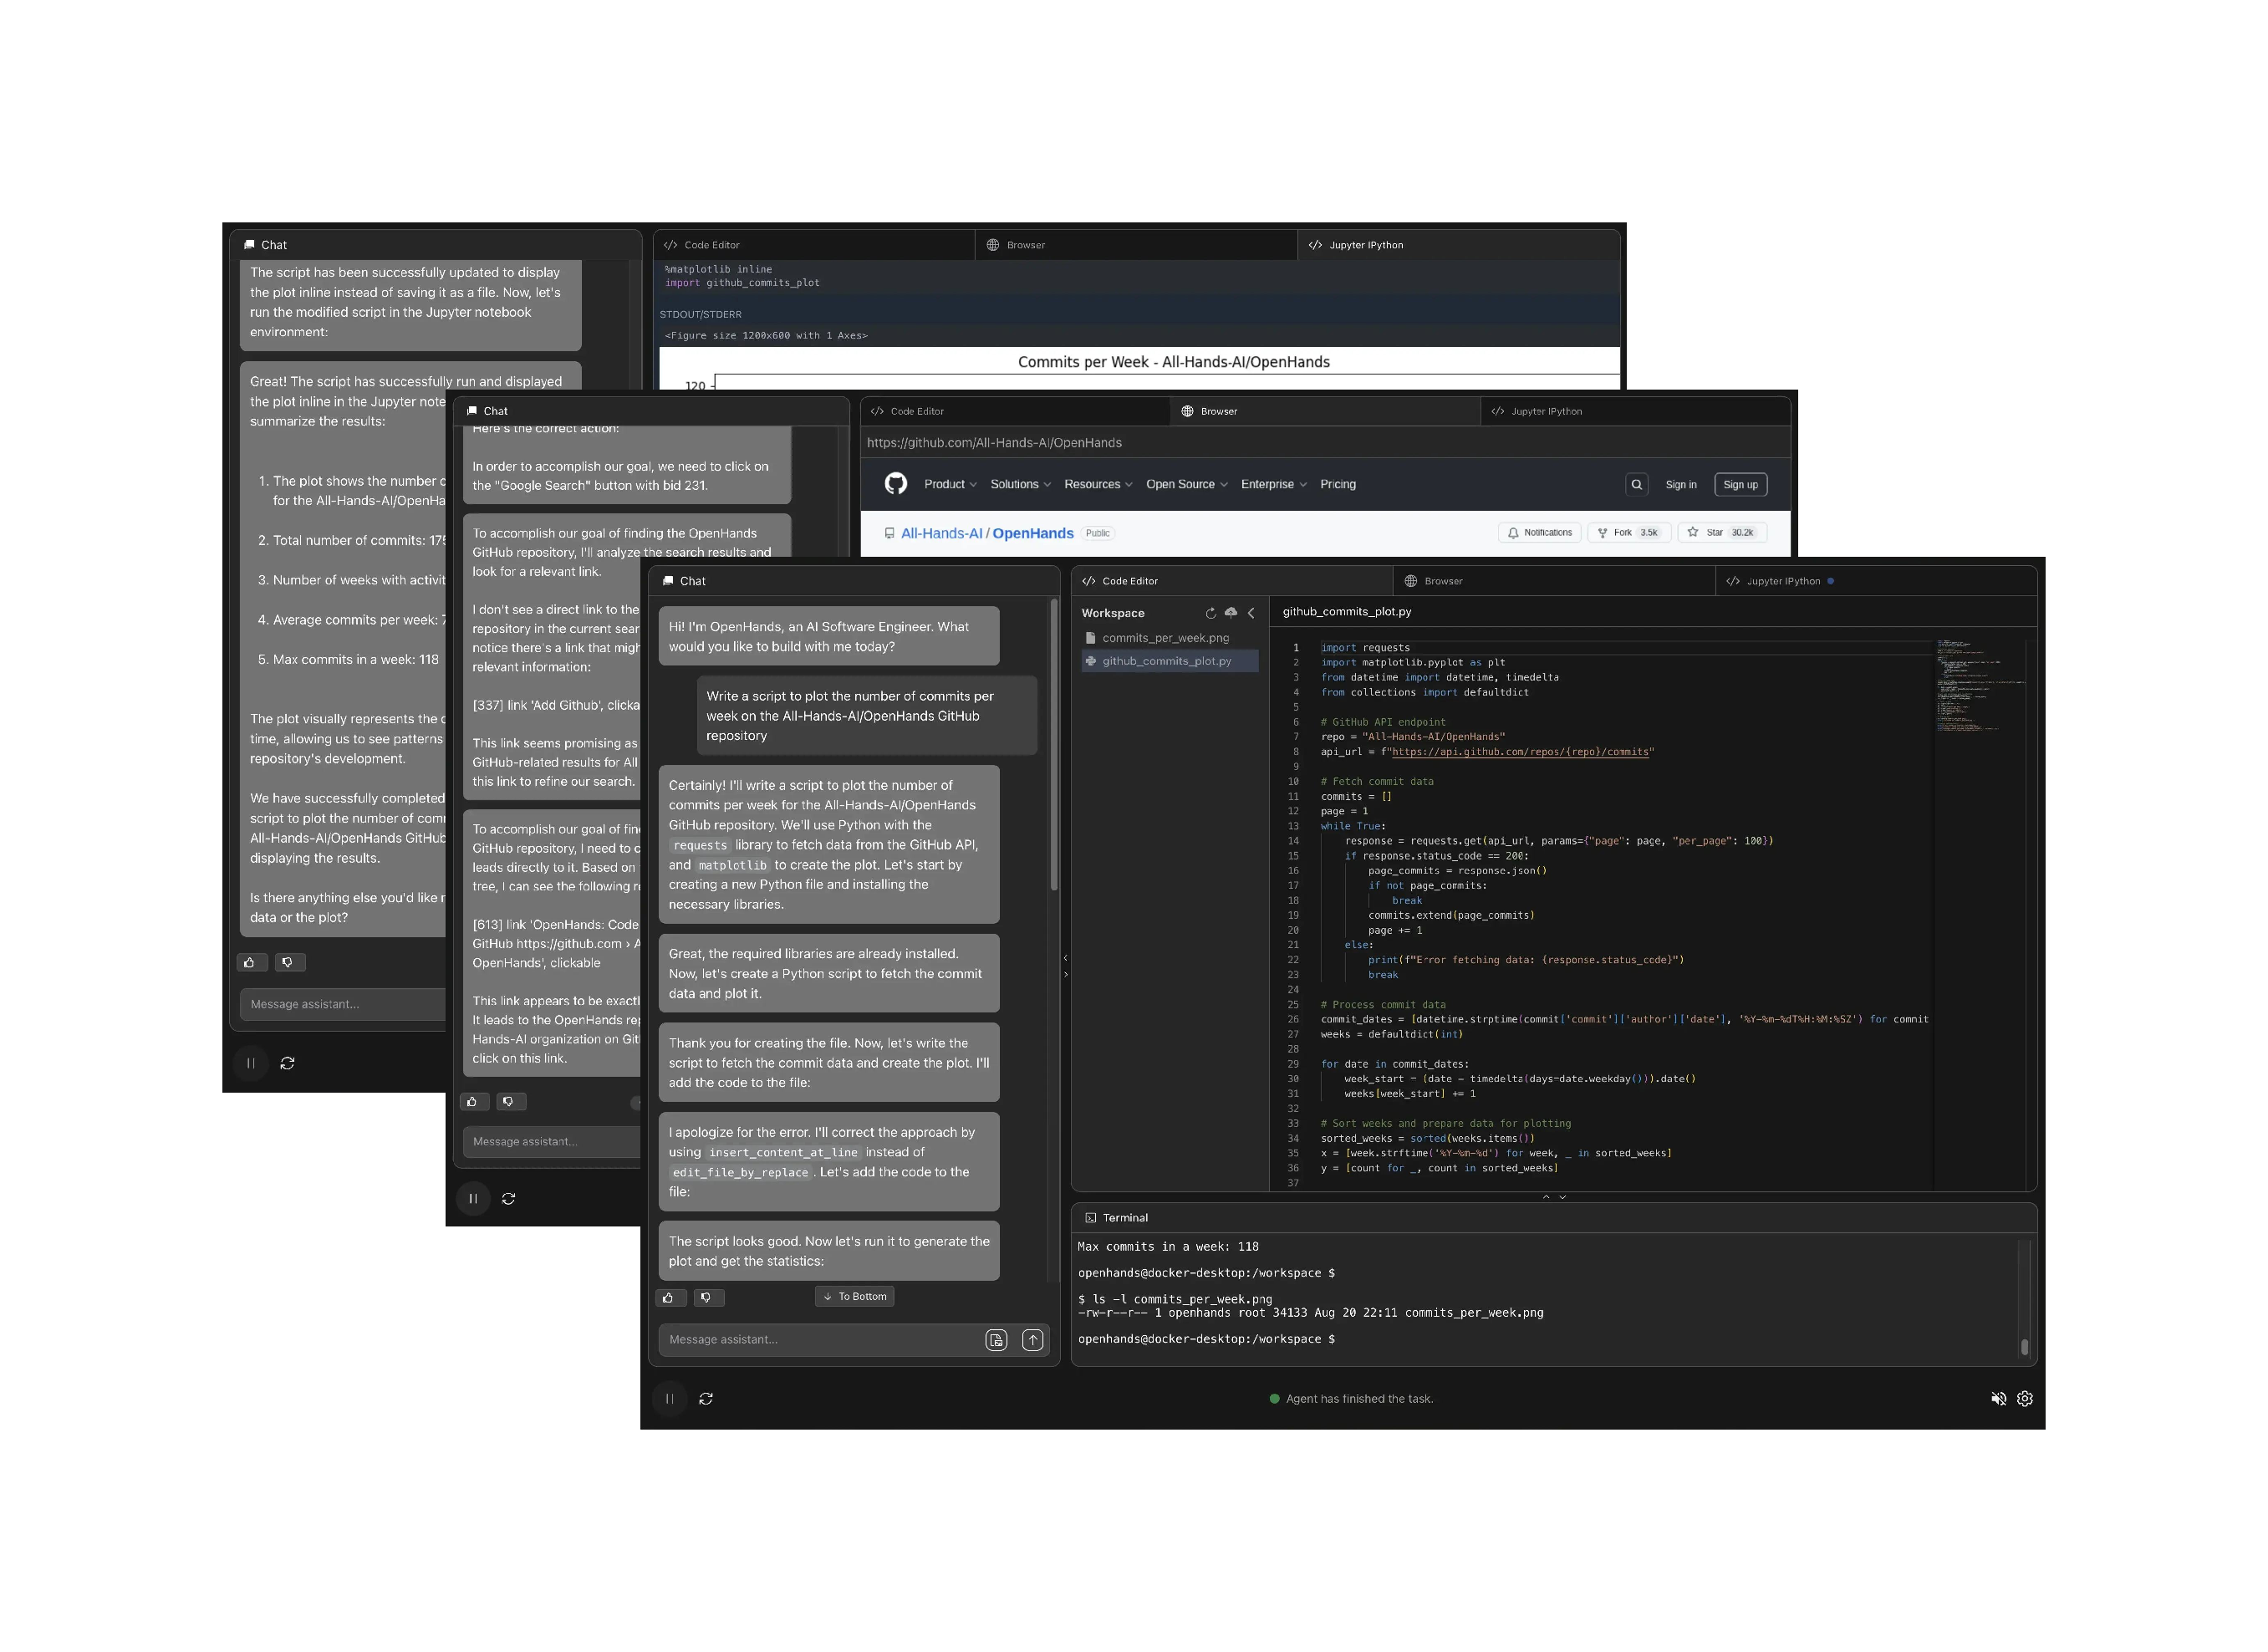
\includegraphics[clip, trim=4.5cm 4.5cm 4.5cm 4.6cm, width=\textwidth]{figs/screenshot-stack.pdf}
\vspace{-0.6cm}
\caption{
\projname User Interface (UI, \sref{sec:ui}) allows users to view files, check executed bash commands/Python code, observe the agent's browser activity, and directly interact with the agent.
}
\label{fig:ui}
\vskip -0.1in
\end{figure}


Importantly, \projname is not just a conceptual framework, but it also includes a comprehensive and immediately usable implementation of agents, environments, and evaluations.
As of this writing, \projname includes an agent hub with over 10 implemented agents (\sref{sec:agenthub}), including a strong generalist agent implemented based on the CodeAct architecture \citep{wang2024executable}, with additions for web browsing \citep{browsergym} and code editing specialists \citep{yang2024sweagent}.
Interaction with users is implemented through a chat-based user interface that visualizes the agent's current actions and allows for real-time feedback (\fref{fig:ui}, \sref{sec:ui}).
Furthermore, the evaluation framework currently supports \numbenchmarks benchmarks, which we use to evaluate our agents (\sref{sec:evaluation}).

Released under a permissive MIT license allowing commercial use,
\projname is poised to support a diverse array of research and real-world applications across academia and industry.
\projname has gained significant traction, with 32K GitHub stars and more than 2.1K contributions from over 188 contributors.
We envision \projname as a catalyst for future research innovations and diverse applications driven by a broad community of practitioners.

